% ============================================================================
% 2026-09-29: the Murphy / threshold analysis and the sample splits parked from
% Section 5.4 (Section~\ref{sec:app_run_parked}: the paper's eight forecasts under
% the session-bar recalibration), re-run for the HEADLINE forecast under the
% 16:00-bar recalibration of Table~\ref{tab:close_option_rules}.  Every number
% below is a macro from generated/appendix_close_murphy_splits.tex, written by
% experiments/close_murphy_splits_headline.py from results/close_murphy_splits/*.csv;
% nothing is typed by hand.  The two recalibrations are never set side by side.
% Input from main.tex after sections/appendix_close_shift_test, so this continues
% Appendix D.
% ============================================================================
% AUTO-GENERATED by experiments/close_murphy_splits_headline.py from results/close_murphy_splits/*.csv -- do not edit.
\begingroup\scriptsize\setlength{\tabcolsep}{2pt}
\begin{longtable}{p{0.27\textwidth}rrrrrrr}
\caption{The comparison set scored two ways on the 866 deck days under the 16:00-bar recalibration: QLIKE against the scorer's target, the elementary score at the trade's threshold (the 15:30 implied variance), the economic loss $|R|\,\mathbf 1\{q\neq\mathrm{sign}(R)\}$, the share of days the forecast falls on the same side of the threshold as the realized variance (same side as $RV$) and the share on which the position has the sign of the settlement return (same side as $R$), and the $\mathrm{sign}(s)$ Sharpe at both fills. The last two rows are rules told the realized variance, and the payoff's sign, in advance.}\label{tab:app_murphy_headline}\\
\toprule
forecast & QLIKE & ES($c{=}1$) & EL & side of $RV$ \% & side of $R$ \% & Sharpe mid & Sharpe crossed \\
\midrule
\endfirsthead
\caption[]{(continued)}\\
\toprule
forecast & QLIKE & ES($c{=}1$) & EL & side of $RV$ \% & side of $R$ \% & Sharpe mid & Sharpe crossed \\
\midrule
\endhead
\bottomrule
\endlastfoot
\textbf{per-bar ridge [live\_feasible]} & 0.101 & 0.100 & 0.349 & 67.4 & 54.7 & 1.90 & 1.44 \\
block-diagonal ridge & 0.106 & 0.100 & 0.380 & 67.2 & 55.0 & 1.00 & 0.53 \\
baseline (HAR + calendar OLS) & 0.117 & 0.099 & 0.374 & 69.7 & 56.6 & 1.17 & 0.69 \\
per-bar lasso [live\_feasible] & 0.096 & 0.096 & 0.351 & 67.8 & 55.1 & 1.83 & 1.36 \\
per-bar ridge [all\_features] & 0.100 & 0.095 & 0.357 & 68.5 & 54.8 & 1.66 & 1.20 \\
per-bar LightGBM [live\_feasible] & 0.098 & 0.105 & 0.356 & 66.2 & 54.6 & 1.69 & 1.22 \\
tuned per-bar LightGBM [all\_features], MSE-selected & 0.101 & 0.107 & 0.352 & 66.4 & 54.6 & 1.81 & 1.35 \\
LSTM live feasible & 0.125 & 0.110 & 0.380 & 63.3 & 53.1 & 1.01 & 0.54 \\
oracle: told RV (sign(RV - slice)) & -- & -- & 0.262 & 100.0 & 62.8 & 4.52 & 4.06 \\
oracle: told the payoff's sign & -- & -- & 0.000 & 62.8 & 100.0 & 17.35 & 17.28 \\
\end{longtable}
\endgroup

\begingroup\scriptsize\setlength{\tabcolsep}{1pt}
\begin{longtable}{llrrrlr}
\caption{Sample splits of the headline's $\mathrm{sign}(s)$ return (midpoint fill) under the 16:00-bar recalibration, beside the paper's block-diagonal ridge scored the same way and always short. $t=\sqrt{n}\,\bar x/s_x$; the Sharpe ratio is annualized with its day-block bootstrap 95\,\% interval (circular blocks of 21 days, 2000 draws); the P\&L share is the split's sum of daily returns over the full-sample sum.}\label{tab:app_splits_headline}\\
\toprule
series & split & $n$ & mean & $t$ & Sharpe [95\,\%] & P\&L share \% \\
\midrule
\endfirsthead
\caption[]{(continued)}\\
\toprule
series & split & $n$ & mean & $t$ & Sharpe [95\,\%] & P\&L share \% \\
\midrule
\endhead
\bottomrule
\endlastfoot
headline sign(s) & all days & 866 & +0.134 & +3.53 & 1.90 [+0.89, +2.94] & 100 \\
headline sign(s) & through 2020-03-31 (the COVID quarter) & 39 & +0.174 & +0.73 & 1.85 [-0.10, +4.02] & 6 \\
headline sign(s) & after 2020-03-31 & 827 & +0.132 & +3.46 & 1.91 [+0.86, +2.99] & 94 \\
headline sign(s) & before 2022-05-16 & 377 & +0.122 & +2.04 & 1.67 [+0.23, +2.90] & 39 \\
headline sign(s) & from 2022-05-16 (daily SPXW listings) & 489 & +0.144 & +2.92 & 2.09 [+0.62, +3.67] & 61 \\
headline sign(s) & settlement pins (R = -1) & 193 & +0.254 & +3.64 & 4.16 [+1.57, +7.33] & 42 \\
headline sign(s) & off pins & 673 & +0.100 & +2.24 & 1.37 [-0.08, +2.71] & 58 \\
reference sign(s) (this scorer) & all days & 866 & +0.071 & +1.86 & 1.00 [-0.03, +2.03] & 100 \\
reference sign(s) (this scorer) & through 2020-03-31 (the COVID quarter) & 39 & -0.116 & -0.48 & -1.22 [-4.86, +0.78] & -7 \\
reference sign(s) (this scorer) & after 2020-03-31 & 827 & +0.080 & +2.08 & 1.15 [+0.10, +2.18] & 107 \\
reference sign(s) (this scorer) & before 2022-05-16 & 377 & +0.063 & +1.05 & 0.86 [-0.80, +2.45] & 38 \\
reference sign(s) (this scorer) & from 2022-05-16 (daily SPXW listings) & 489 & +0.077 & +1.56 & 1.12 [-0.11, +2.44] & 62 \\
reference sign(s) (this scorer) & settlement pins (R = -1) & 193 & +0.285 & +4.12 & 4.71 [+1.23, +8.47] & 89 \\
reference sign(s) (this scorer) & off pins & 673 & +0.010 & +0.22 & 0.13 [-1.20, +1.29] & 11 \\
always short & all days & 866 & +0.014 & +0.38 & 0.20 [-0.62, +1.16] & 100 \\
always short & through 2020-03-31 (the COVID quarter) & 39 & -0.302 & -1.28 & -3.25 [-6.76, +0.59] & -94 \\
always short & after 2020-03-31 & 827 & +0.029 & +0.76 & 0.42 [-0.34, +1.41] & 194 \\
always short & before 2022-05-16 & 377 & -0.033 & -0.55 & -0.45 [-1.52, +0.84] & -98 \\
always short & from 2022-05-16 (daily SPXW listings) & 489 & +0.051 & +1.02 & 0.73 [-0.35, +1.93] & 198 \\
always short & settlement pins (R = -1) & 193 & +1.000 & -- & --  & 1540 \\
always short & off pins & 673 & -0.268 & -6.15 & -3.77 [-4.64, -2.85] & -1440 \\
\end{longtable}
\endgroup

\newcommand{\hmurHQLIKE}{0.101}
\newcommand{\hmurHES}{0.100}
\newcommand{\hmurHQLIKERankSet}{4}
\newcommand{\hmurHESRankSet}{4}
\newcommand{\hmurHQLIKERankAll}{63}
\newcommand{\hmurHESRankAll}{41}
\newcommand{\hmurHSharpeRankAll}{4}
\newcommand{\hmurNAll}{115}
\newcommand{\hmurNSet}{8}
\newcommand{\hmurHHitVar}{67}
\newcommand{\hmurHHitPay}{55}
\newcommand{\hmurHTop}{14}
\newcommand{\hmurOracleAgree}{63}
\newcommand{\hmurOracleMiss}{37}
\newcommand{\hmurOracleShMid}{4.52}
\newcommand{\hmurOracleShX}{4.06}
\newcommand{\hmurPayoffOracleShX}{17.28}
\newcommand{\hmurLeaderAtOne}{per-bar ridge [all\_features]}
\newcommand{\hmurHRankAtOne}{4}
\newcommand{\hmurNGrid}{33}
\newcommand{\hmurNLeadH}{13}
\newcommand{\hmurNLeadLin}{25}
\newcommand{\hmurGridMin}{0.25}
\newcommand{\hmurGridMax}{4}
\newcommand{\hmurRhoQSet}{+0.67}
\newcommand{\hmurRhoQSetLo}{+0.07}
\newcommand{\hmurRhoQSetHi}{+0.90}
\newcommand{\hmurRhoESSet}{+0.24}
\newcommand{\hmurRhoESSetLo}{-0.52}
\newcommand{\hmurRhoESSetHi}{+0.76}
\newcommand{\hmurRhoQAll}{+0.65}
\newcommand{\hmurRhoQAllLo}{+0.13}
\newcommand{\hmurRhoQAllHi}{+0.74}
\newcommand{\hmurRhoESAll}{+0.58}
\newcommand{\hmurRhoESAllLo}{+0.15}
\newcommand{\hmurRhoESAllHi}{+0.77}
\newcommand{\hsplHAllSh}{1.90}
\newcommand{\hsplHAllT}{3.53}
\newcommand{\hsplNCovid}{39}
\newcommand{\hsplHPostCovidN}{827}
\newcommand{\hsplHPostCovidSh}{1.91}
\newcommand{\hsplHPostCovidT}{3.46}
\newcommand{\hsplHPostCovidLo}{0.86}
\newcommand{\hsplHPostCovidHi}{2.99}
\newcommand{\hsplHPreN}{377}
\newcommand{\hsplHPreSh}{1.67}
\newcommand{\hsplHPreT}{2.04}
\newcommand{\hsplHPreLo}{0.23}
\newcommand{\hsplHPreHi}{2.90}
\newcommand{\hsplHPostN}{489}
\newcommand{\hsplHPostSh}{2.09}
\newcommand{\hsplHPostT}{2.92}
\newcommand{\hsplHPostLo}{0.62}
\newcommand{\hsplHPostHi}{3.67}
\newcommand{\hsplRPreSh}{0.86}
\newcommand{\hsplRPostSh}{1.12}
\newcommand{\hsplNPin}{193}
\newcommand{\hsplPinPct}{22.3}
\newcommand{\hsplHPinMean}{+0.25}
\newcommand{\hsplHOffPinMean}{+0.10}
\newcommand{\hsplHPinShare}{42}
\newcommand{\hsplASOffPinMean}{-0.27}
\newcommand{\hsplASPinMean}{+1.00}
\newcommand{\hsplSignBuyMean}{+0.15}
\newcommand{\hsplSignSellMean}{-0.12}
\newcommand{\hsplSignDiff}{0.27}
\newcommand{\hsplSignT}{3.28}
\newcommand{\hsplSignNBuy}{348}
\newcommand{\hsplSignNSell}{518}

\subsection{The Headline Forecast Scored at the Trade's Threshold, and Its Sample Splits}
\label{sec:app_murphy_splits_headline}

\paragraph{The score at the threshold.} Section~\ref{sec:app_run_parked} takes QLIKE
apart by threshold (Equations~\eqref{eq:elementary_score}--\eqref{eq:score_at_threshold})
and reads the trade at the one threshold it uses, the day's implied variance of the last
half hour. Table~\ref{tab:app_murphy_headline} repeats that scoring under the 16:00-bar
recalibration for a comparison set of \hmurNSet{} forecasts --- the headline, the paper's
block-diagonal ridge scored the same way, the HAR $+$ calendar least squares, the
headline's lasso twin, the all-features ridge, an untuned and a tuned tree, and the
LSTM --- and \texttt{scores\_by\_forecast.csv} carries all \hmurNAll{} forecasts of the
master table. QLIKE is against the scorer's target; the identity between QLIKE and the
$\theta^{-2}$ mixture of elementary scores is checked day by day for the headline, and
the identity $\overline{qR}=\overline{|R|}-2\,\overline{EL}$ for every forecast. The
headline scores \hmurHQLIKE{} on QLIKE and \hmurHES{} at the threshold, ranking
\hmurHQLIKERankSet{} and \hmurHESRankSet{} of \hmurNSet{} in the set (\hmurHQLIKERankAll{}
and \hmurHESRankAll{} of \hmurNAll{} overall; its crossed-spread Sharpe ratio ranks
\hmurHSharpeRankAll{} of \hmurNAll{}). It falls on the realized variance's side of the
threshold on \hmurHHitVar{}\,\% of days and on the payoff's side on \hmurHHitPay{}\,\%,
and it is long on \hmurHTop{} of the 20 best long-straddle days.

\paragraph{The Murphy diagram.} Figure~\ref{fig:app_murphy_headline} plots the mean
elementary score against the threshold, in units of the implied variance, from
\hmurGridMin{} to \hmurGridMax{} on a logarithmic grid of \hmurNGrid{} points. The headline
has the lowest score of the set at \hmurNLeadH{} of the \hmurNGrid{} thresholds and a
linear forecast at \hmurNLeadLin{}; at the trade's threshold the leader is
\hmurLeaderAtOne{} and the headline ranks \hmurHRankAtOne{} of \hmurNSet{}.

\paragraph{What a variance forecast can reach.} A rule told the realized variance in
advance takes the payoff's side on \hmurOracleAgree{}\,\% of days (Sharpe
\hmurOracleShMid{} at the midpoint, \hmurOracleShX{} across the spread), against
\hmurPayoffOracleShX{} across the spread for a rule told the payoff's sign; on
\hmurOracleMiss{}\,\% of days the trade's sign is beyond any variance forecast.

\paragraph{Which score orders the forecasts on the trade.} Across the comparison set
the rank correlation of minus the loss with the crossed-spread Sharpe ratio is
\hmurRhoQSet{} for QLIKE (day-block bootstrap 95\,\% interval \hmurRhoQSetLo{} to
\hmurRhoQSetHi{}) and \hmurRhoESSet{} for the score at the threshold (\hmurRhoESSetLo{} to
\hmurRhoESSetHi{}); across all \hmurNAll{} forecasts of the master table it is
\hmurRhoQAll{} (\hmurRhoQAllLo{} to \hmurRhoQAllHi{}) and \hmurRhoESAll{} (\hmurRhoESAllLo{}
to \hmurRhoESAllHi{}). The economic loss is affine in the midpoint P\&L and correlates
perfectly by construction; it is reported as the ceiling.

\paragraph{Sample splits.} Table~\ref{tab:app_splits_headline} repeats the splits of
Section~\ref{sec:app_run_parked} for the headline's $\mathrm{sign}(s)$ return, beside
the paper's forecast scored the same way and always short. Over all 866 days the
headline's annualized Sharpe ratio is \hsplHAllSh{} ($t=\hsplHAllT$). Dropping the
\hsplNCovid{} expiration days through 31~March~2020 leaves \hsplHPostCovidSh{}
($t=\hsplHPostCovidT$, interval \hsplHPostCovidLo{} to \hsplHPostCovidHi{}) on the
remaining \hsplHPostCovidN{} days. Split at 16~May~2022, when SPXW listings became
daily, it is \hsplHPreSh{} ($t=\hsplHPreT$, \hsplHPreLo{} to \hsplHPreHi{}) on the
\hsplHPreN{} days before and \hsplHPostSh{} ($t=\hsplHPostT$, \hsplHPostLo{} to
\hsplHPostHi{}) on the \hsplHPostN{} days after; the paper's forecast scored the same way
reads \hsplRPreSh{} and \hsplRPostSh{}. The straddle expires worthless on \hsplNPin{} of
the days (\hsplPinPct{}\,\%): always short collects \hsplASPinMean{} on them against
\hsplASOffPinMean{} elsewhere, and the headline averages \hsplHPinMean{} on them against
\hsplHOffPinMean{} off them, so pin days supply \hsplHPinShare{}\,\% of its total return.
Read as a same-day sign split, the settlement return averages \hsplSignBuyMean{} on the
\hsplSignNBuy{} days the headline buys and \hsplSignSellMean{} on the \hsplSignNSell{}
days it sells (difference \hsplSignDiff{}, heteroskedasticity-robust $t=\hsplSignT$).

\begin{figure}[H]
\centering
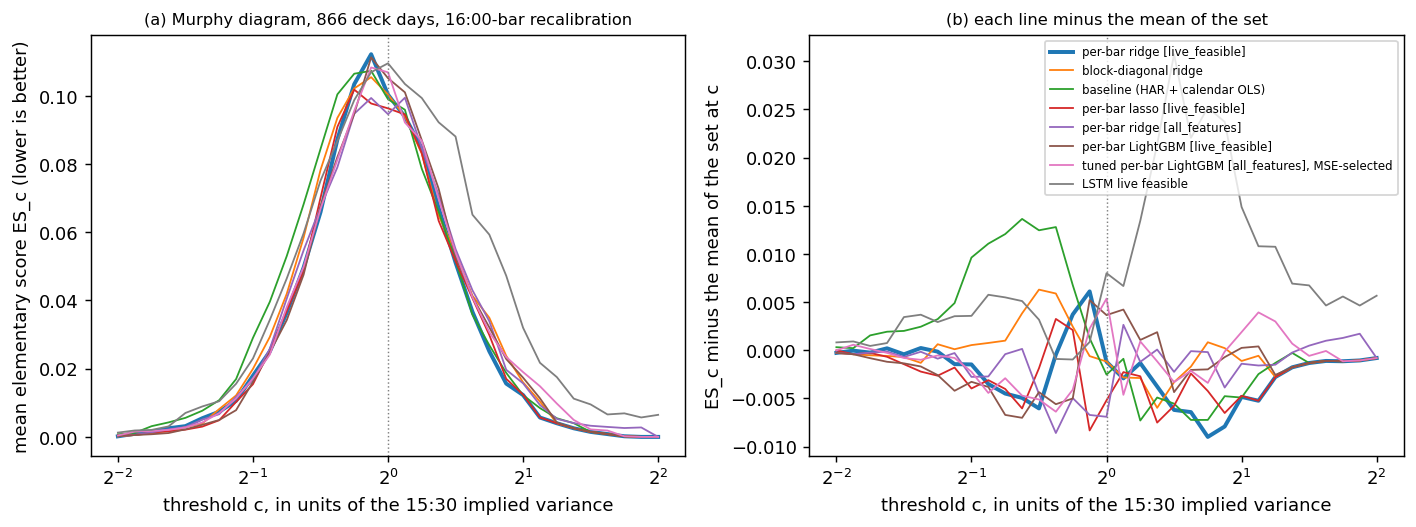
\includegraphics[width=\textwidth]{../results/close_murphy_splits/murphy_headline.png}
\caption{Murphy diagram of the comparison set on the 866 deck days under the 16:00-bar
recalibration. The horizontal axis is the threshold in units of the day's implied
variance of the last half hour, on a logarithmic scale from \hmurGridMin{} to
\hmurGridMax{}; the dotted line at 1 is the threshold the $\mathrm{sign}(s)$ rule uses.
(a) The mean elementary score (lower is better); QLIKE is the area under each line
weighted by $c^{-2}$. (b) Each line minus the mean of the set at the same threshold
(source: \texttt{results/close\_murphy\_splits/murphy\_grid.csv}).}
\label{fig:app_murphy_headline}
\end{figure}
